\documentclass[11pt,a4paper]{article}
\usepackage[utf8]{inputenc}
\usepackage[spanish]{babel}
\usepackage{amsmath}
\usepackage{amsfonts}
\usepackage{amssymb}
\usepackage{graphicx}
\usepackage[left=2cm,right=2cm,top=2cm,bottom=2cm]{geometry}
\usepackage{hyperref}

\author{Grupo Los Walo}
\title{Algoritmo de Búsqueda Indexada}
\date{19 de julio de 2013}


\begin{document}
\maketitle

\begin{abstract}
En este articulo se enuncian una descripción del método,las principales características que tiene el método de búsqueda indexada, sus ventajas , desventajas y algunas aplicaciones que operan con el método mencionado.
\end{abstract}

\section{Introducción}
Los métodos de búsqueda nos permiten recuperar información de un vector o un archivo,
que contenga una lista de datos. Por ejemplo se puede obtener el nombre y el número
telefónico de nuestra agenda de contactos o la nota obtenida por un alumno en la lista de
un curso.
Cuando se realizan búsquedas sobre vectores, se desea es encontrar la posición que
ocupa el elemento buscado dentro de la lista de elementos que contiene el vector. Para la
búsqueda de información en archivos es necesario realizar la búsqueda a partir de un
campo clave dentro del archivo.
Existen diferentes métodos de búsqueda y se puede determinar con cual método trabajar
dependiendo de la cantidad de elementos que existan en el vector o la organización de
dichos elementos.
A continuación se describirá el método búsqueda indexada.

\section{Estudio del arte}
Los algoritmos de búsqueda aparecen por los años 1968, con el algoritmo de búsqueda A (pronunciado "A asterisco" o "A estrella") se clasifica dentro de los algoritmos de búsqueda en grafos. Presentado por por Peter E. Hart, Nils J. Nilsson y Bertram Raphael, el algoritmo A* la ruta de menor coste entre dos puntos siempre y cuando se
cumplan una serie de condiciones.Está clasificado dentro de los algoritmos de búsqueda
en grafos ya que tiene la necesidad de dar a los mecanismos robóticos, vehiculares o
virtuales un sistema de navegación autónomo.
Luego van apareciendo otros algoritmos, aparece un algoritmo llamado algoritmo de búsqueda de cadenas Boyer-Moore es un particularmente eficiente algoritmo de búsqueda de cadenas, y ha sido el punto de referencia estándar para la literatura de búsqueda de cadenas. Fue desarrollado por Bob Boyer y J Strother Moore en 1977. El algoritmo pre procesa la cadena objetivo (clave) que está siendo buscada, pero no en la cadena en que se busca (no como algunos algoritmos que procesan la cadena en que se busca y pueden entonces amortizar el coste del pre procesamiento mediante búsqueda repetida). El tiempo de ejecución del algoritmo Boyer-Moore, aunque es lineal en el tamaño de la cadena que esta siendo buscada, puede tener un factor significativamente más bajo que muchos otros algoritmos de búsqueda: no necesita comprobar cada carácter de la cadena que es buscada, puesto que salta algunos de ellos. Generalmente el algoritmo es más rápido cuanto más grande es la clave que es buscada, usa la información conseguida desde un intento para descartar tantas posiciones del texto como sean posibles en donde la cadena no coincida.\\
Y así entre algunos hasta llegar a los que son mas conocidos como búsqueda secuencial , secuencial indexada,búsqueda binaria,hash(Ver Fig.\ref{figmet}).

\begin{figure}
\centering
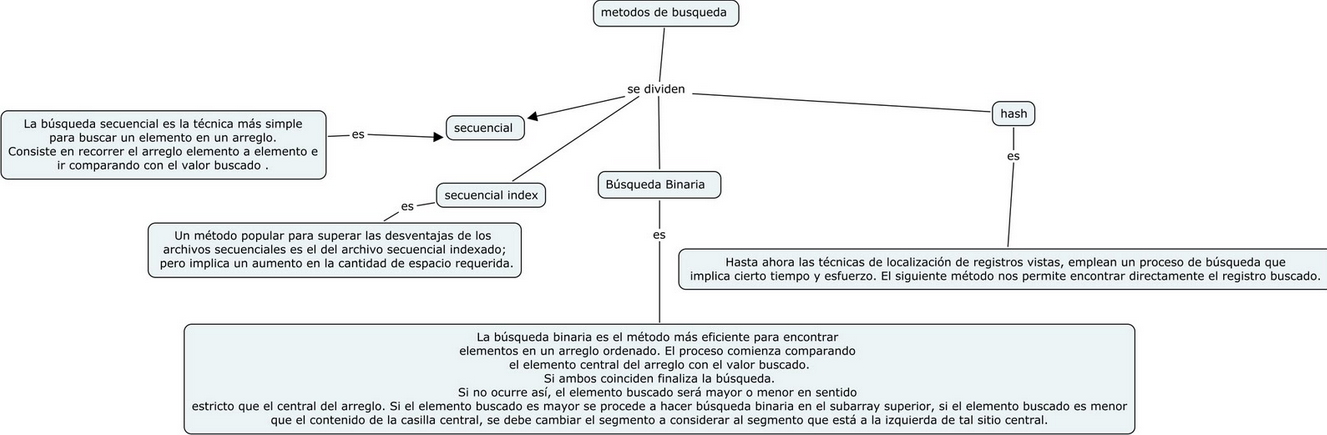
\includegraphics[scale=0.5]{clasif}
\caption{Clasificación de los métodos de búsqueda}
\label{figmet}
\end{figure}

\section{Descripción de la búsqueda indexada}
En este modo de organización, al fichero le acompaña un fichero de índice que tiene la función de permitir el acceso directo a los registros del fichero de datos. El índice se puede organizar de diversas formas, las más típicas son: secuencial, multinivel y árbol. A través del índice podremos procesar un fichero de forma secuencial o de forma directa según la clave de indexación, y esto independientemente de cómo esté organizado el fichero por sí mismo. El índice debe estar organizado en función de alguno de los campos de los registros de datos. Se pueden tener tantos índices como se quiera variando la clave (o campo) que se emplee. El índice está formado por registros (entradas) que contienen:

\begin{itemize}
\item Clave de organización.
\item Puntero(s) al fichero de datos, en concreto al registro que corresponda.
\end{itemize}

\section{Técnica de búsqueda secuencial indexada}
\subsection{Descripción de la técnica}
Funciona de la siguiente manera:\\ \\
Se reserva una taba auxiliar llamada índice además del archivo ordenado mismo. Cada elemento en el índice consta de una llave kindex y un apuntador al registro en el archivo que corresponde a kindex. Los elementos en el índice al igual que los elementos en el archivo, deben estar ordenados en la llave. Si el índice es de un octavo del tamaño del archivo, se representa en el índice cada octavo que registra el archivo(Ver Fig.\ref{figIndex}).

\subsection{Indexacion y búsqueda(Accesos a datos)}
Para aumentar la eficiencia de acceso e indexación se diseñan estructuras adicionales asociadas a los archivos que mantienen la información de las bases de datos.

Existen distintas formas generales para la indexación y búsqueda. Cada una de las técnicas tiene ventajas y desventajas comparativas y deben evaluarse de a cuerdo a:

\newpage

\begin{itemize}
\item tiempo de acceso a datos.
\item tiempo de inserciónn de datos.
\item tiempo de eliminación de datos.
\item espacio extra necesario para la indexación de más terminología.
\end{itemize}

La idea de crear indices y realizar su posterior indexación es la misma que en el caso de un índice de un libro, en este existe un indice alfabético y permite ir directamente a la página asociada con cada entrada del índice, al igual existen varias bibliotecas que mantienen fichas en las cuales la indexación es realizada por tema, título y autor, que entregan la información relacionada acerca de en donde se encuentra, osea el estante, el número del libro para ser encontrarlo fácilmente.

El índice define los atributos que tiene cada uno de los términos para asociarla a una relación de contenidos y da valor a todos lo bloques de información que contienen dicho término.

Los valores en la indexación se mantienen con cierto orden de modo que se pueda realizar la búsqueda rapidamente.

Existen entonces distintas técnicas de indexación con distintas características.

\begin{itemize}
\item Indexación por árboles de términos
\item Indexación por archivos de términos secuenciales
\end{itemize}


\begin{figure}
\centering
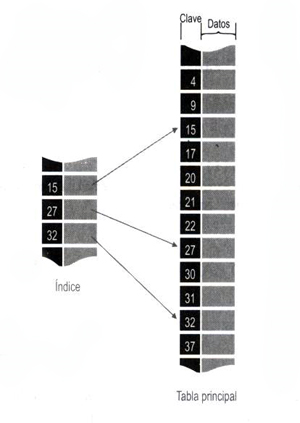
\includegraphics[scale=0.7]{Index}
\caption{Ilustración de indice con su tabla principal}
\label{figIndex}
\end{figure}

Si el índice comienza a crecer tanto que se vuelve ineficaz se puede usar un índice secundario que funciona casi de la misma forma que el índice principal, solo que apunta a este, no a la tabla principal la búsqueda empieza con una exploración por el índice secundario; esto nos lleva a un subarreglo en el índice principal; después el procesamiento continua normalmente. Un ejemplo de lo anterior es la siguiente figura:(Ver Fig.\ref{figIndex2})

\begin{figure}
\centering
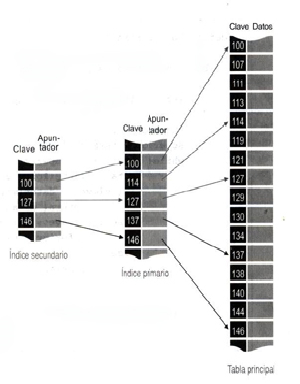
\includegraphics[scale=0.7]{Index2}
\caption{Uso de indice secundario cuando crece mucho el indice primario}
\label{figIndex2}
\end{figure}

\subsection{Indexacion por acceso secuencial}
Es uno de los esquemas de indexación mas antiguos que existen para realizar una búsqueda ordenada. Este tipo de indexación expone el ordenamiento secuencial y que por lo tanto tendrán una llave de búsqueda primaria. Es por lo tanto que en este aparte caben destacar dos tipos de índices:

\newpage

\begin{itemize}
\item Indice denso: Este indice se refiere cuando el archivo índice contiene la dirección de cada
registro de la llave.
\item Indice disperso : Este indice se refiere cuando el archivo índice contiene la dirección de cada registro de la llave.
\end{itemize}

Resulta entonces que entre más pequeño sea el índice la indexación y búsqueda resultara más rápida, dado que la terminología utilizada sera la misma porque se realizan asociaciones dentro del motor de búsqueda. 

Sin importar cuál sea la forma de indexación siempre se debe actualizar todos los índices cada vez que se inserta o elimina una palabra (término).

Cabe destacar que entre más datos tengan los contenidos más cuesta acceder, manipular y no facilita la búsqueda de la información.

La indexación sera ineficiente si se realizan muchas inserciones o eliminaciones.

Se pueden indexar atributos a aquellos términos que no se encuentran secuencialmente ordenados, como palabras compuestas utilizando etiquetas que direccionen la búsqueda y recuperación de información.

\section{Ventajas y desventajas de la búsqueda indexada}
\section*{Ventajas}
Permite procesar el archivo secuencialmente por orden lógico y también procesarlo al azar.
La ventaja real del método secuencial indexado es que los elementos en la tabla pueden ser examinados en forma secuencial si todos los registros en el archivo deben ser accesados, pero sin embargo, el tiempo de búsqueda para algún elemento en particular se reduce considerablemente. La búsqueda secuencial se realiza en la tabla de índices que es más pequeña en lugar de la tabla más grande. Una vez que se ha encontrado un índice correcto, se hace una segunda búsqueda secuencial únicamente en la parte reducida de la tabla que contiene los registros.
La organización secuencial indexada es conveniente para archivos con mediana volatilidad, actividad variable y tamaño relativamente estable.
Las eliminaciones de una tabla secuencial indexada se pueden hacer fácilmente mediante la asignación de banderas a las entradas que son eliminadas. Durante la búsqueda secuencial a través de la tabla, se ignoran las entradas que han sido eliminadas.

\section*{Desventajas}
Implica un aumento en la cantidad de espacio requerida, porque se ocupa un índice y “se pone a un lado además del fichero clasificado a sí mismo”.
La inserción en una tabla secuencial indexada es un poco más difícil debido a que puede qe no exista espacio entre dos entradas en la tabla, siendo necesario mover un gran número de elementos en la tabla.
El uso de una lista ligada (índice) da una gran sobrecarga de espacio y tiempo para los apuntadores que se utilizan en la búsqueda de registros.
Los registros deben ser de longitud fija. El archivo debe estar soportado por una memoria de masa tal como el disco; no se utiliza en cinta magnética. A veces todo el archivo debe estar presente en línea.

\section{Reglas de indexacion}
La regla principal a respetar es utilizar un número limitado de palabras clave (ni demasiadas, ni demasiado pocas). Según el tipo de información que se quiera describir, se  pueden necesitar varias palabras clave, pero no muchas.
\\
Cuantas menos palabras clave se usen, más relevantes son. Este es el modo en que los motores de búsqueda tienen en cuenta a la hora de la relevancia en los términos y por ende la importancia que toma cada uno a la hora de la búsqueda.También es importante el orden de las palabras clave y ordenarlas correctamente.
\\\\
La palabra clave más relevante debe ir primero. Determinará el lugar en la página de resultados. Si la primera palabra clave no es la más pertinente, el contenido puede no aparecer cuando es necesitado.

Se deben indexar los términos en un solo idioma, ya que el motor de búsqueda traduce automáticamente todas las palabras clave en todos los idiomas disponibles en el sitio web. Si se utilizan idiomas diferentes en la indexación, el archivo no puede ser tenido en cuenta para búsquedas específicas. La precisión es también un punto importante de la indexación, y se deben utilizar sólo palabras clave que describan el contenido. No se deben encontrar todos los sinónimos posibles para un solo concepto, y está absolutamente prohibido utilizar palabras clave que no están ligadas directamente al concepto por representar.

Para tener una buena indexación también se deben respetar algunas pautas semánticas que ayudarán a que el contenido aparezca en el lugar correcto en el momento oportuno.

Las palabras compuestas serán escritas de una vez (en la misma línea), especialmente cuando el significado de las palabras tomadas separadamente sea muy diferente de la palabra compuesta.

El uso del plural será limitado a los términos que representan efectivamente varias veces el sujeto. Es lo mismo para singular; no se debe poner la palabra clave en singular si el sujeto es representado varias veces.

Cada una de estas especificaciones son importantes porque determinarán la visibilidad del contenido y su potencial o relevancia. Si no se respetan ciertas indicaciones la relevancia de las palabras clave disminuirá y no se adecuarán a los hábitos de búsqueda de los usuarios.

Cuando un usuario busca un término o concepto, él ya sabe lo que quiere hacer. Generalmente escribe una palabra clave representativa, por eso es importante ser muy preciso durante la indexación.


\section{Principales aplicaciones}
Un uso en la cual esta búsqueda se aplica, es donde se presenta el ingreso de datos (registros) sin ningún tipo de orden especifico; pero en cada determinado momento su campo llave es almacenado en un índice, en el cual esas llaves están ordenadas de menor a mayor o de mayor a menor dependiendo el uso que se le de. De esta manera, para agilizar la búsqueda de un registro en particular se acceso a ese registro por medio de su campo llave almacenado en el índice.
Un ejemplo de nuestra vida diaria y donde se aplica esta búsqueda es en un negocio mediano (negocio de carnes frías, refaccionaria), ya que aquí se necesita una búsqueda eficiente con una sola clave de acceso y otorgándonos la información requerida.


\begin{thebibliography}{03}
\bibitem{Wikipedia} Wikipedia: \url{http://es.wikipedia.org/wiki/Indexaci%C3%B3n}
\bibitem{novella} novella: \url{http://novella.mhhe.com/sites/dl/free/844814077x/619434/A06.pdf}
\bibitem{trevinca} trevinca: \url{http://trevinca.ei.uvigo.es/~rlaza/teoria/Tema2_Transparencias.pdf}

\end{thebibliography}






\end{document}